% !TEX TS-program = pdflatex
% !TeX program = pdflatex
% !TEX encoding = UTF-8
% !TEX spellcheck = fr

\documentclass[xcolor=table]{beamer}


%\usepackage{fullpage}
%\usepackage[left=2.8cm,right=2.2cm,top=2 cm,bottom=2 cm]{geometry}
\setbeamersize{text margin left=10pt,text margin right=10pt}


\usepackage{amsmath,amssymb} 
\usepackage{fontenc}
\usepackage{textcomp}
\usepackage[utf8]{inputenc}
\usepackage{CJKutf8}
\usepackage[french]{babel}
\usepackage{arabtex,acolor}
\usepackage{txfonts}
\usepackage{tipa}
\usepackage[]{graphicx}
\usepackage{multirow}
\usepackage{hyperref}
\usepackage{colortbl}
\usepackage{tabularray}
\usepackage{listingsutf8}
\usepackage{wrapfig}
\usepackage{multicol}
\usepackage[export]{adjustbox} %for images in table, also for frame
\usepackage[many]{tcolorbox}
\usepackage{wasysym}
\usepackage[french,lined]{algorithm2e}
\usepackage{alltt} %verbatim with commands
\usepackage{longtable}
\usepackage{tabu}


\definecolor{lightblue}{HTML}{D0D2FF}
\definecolor{lightyellow}{HTML}{FFFFAA}
\definecolor{darkblue}{HTML}{0000BB}
\definecolor{olivegreen}{HTML}{006600}
\definecolor{darkgreen}{HTML}{008B45} %009B55
\definecolor{violet}{HTML}{6600CC}
%\definecolor{deeppink}{HTML}{FF1493}
\definecolor{orangey}{HTML}{FFBB00}

\usetheme{Warsaw} % Antibes Boadilla Warsaw

\beamertemplatenavigationsymbolsempty


\let\oldcite\cite
\renewcommand{\cite}[1]{{\bfseries\color{orangey}\oldcite{#1}}}

\tcbuselibrary{listings}

\newcommand{\kurl}[1]{{\scriptsize\bfseries\color{orangey}\url{#1}}}


%\renewcommand{\baselinestretch}{1.5}

\def\supit#1{\raisebox{0.8ex}{\small\it #1}\hspace{0.05em}}

\AtBeginSection{%
	\begin{frame}
		\sectionpage
	\end{frame}
}

\newcommand{\rottext}[2]{%
	\rotatebox{90}{%
	\begin{minipage}{#1}%
		\raggedleft#2%
	\end{minipage}%
	}%
}


\institute{ %
Laboratoire de la Communication dans les Systèmes Informatiques (LCSI)

\vspace{6pt}
École  nationale Supérieure d'Informatique (ESI, ex. INI), Alger, Algérie
}
\author[ \textbf{\footnotesize\insertframenumber/\inserttotalframenumber} \hspace*{1cm} ESI - ARIES Abdelkrime (Master 2022/2023)] %
{ARIES Abdelkrime}
%\titlegraphic{
\includegraphics[height=1cm]{../img/esi-logo.png}%\hspace*{4.75cm}~
	
	
	\date{Master 2022/2023} %\today

\titlegraphic{%
	
\includegraphics[height=1cm]{../img/esi-logo.png}%
	\hspace{2cm}
	
\includegraphics[height=1cm]{../img/lcsi-logo.png}%
}


%\setbeamertemplate{headline}{}



\newcommand{\keyword}[1]{\textcolor{red}{\bfseries\itshape #1}}
\newcommand{\expword}[1]{\textcolor{olivegreen}{#1}}
\newcommand{\optword}[1]{\textcolor{violet}{\bfseries #1}}

\makeatletter
\newcommand\mysphere{%
	\parbox[t]{10pt}{\raisebox{0.2pt}{\beamer@usesphere{item projected}{bigsphere}}}}
\makeatother

%\let\oldtabular\tabular
%\let\endoldtabular\endtabular
%\renewenvironment{tabular}{\rowcolors{2}{white}{lightblue}\oldtabular\rowcolor{blue}}{\endoldtabular}


\NoAutoSpacing %french autospacing after ":"

\def\graphpath{}

\newcommand{\changegraphpath}[1]{\def\graphpath{#1}}


\newcommand{\vgraphpage}[2][.84\textheight]{%
%	\begin{center}%
		\includegraphics[height=#1]{\graphpath #2}%
%	\end{center}%
}

\newcommand{\hgraphpage}[2][\textwidth]{%
%	\begin{center}%
		\includegraphics[width=#1]{\graphpath #2}%
%	\end{center}%
}

\newcommand{\graphpage}[2][]{%
	\includegraphics[#1]{\graphpath #2}%
}

\bibliographystyle{apalike}

\newcommand{\insertbibliography}[2]{
	\appendix
	\section*{Bibliographie}
	\nocite{#2}
%	\makeatletter % to change template
%	\setbeamertemplate{headline}[default] % not mandatory, but I though it was better to set it blank
%	\def\beamer@entrycode{\vspace*{-\headheight}} % here is the part we are interested in :)
%	\makeatother
	\begin{multicols*}{2}[\frametitle{\insertsection} \usebeamertemplate*{frametitle}]%\usebeamertemplate*{frametitle}\frametitle{Références}
		\tiny
		\bibliography{#1}
	\end{multicols*}
}

\definecolor{my-grey}{RGB}{233, 233, 233}

\newcommand{\insertlicence}{
	\begin{frame}[plain]
	\frametitle{Licence : CC-BY 4.0}
%	\framesubtitle{Licence: CC-BY-NC 4.0}

	\begin{tcolorbox}[colback=cyan,
		colframe=cyan,  
		arc=0pt,outer arc=0pt,
		valign=top, 
		halign=center,
		width=\textwidth]
		
		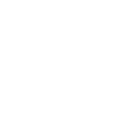
\includegraphics[width=.5cm]{../img/licence/cc_icon_white_x2.png}
		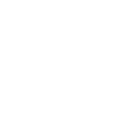
\includegraphics[width=.5cm]{../img/licence/attribution_icon_white_x2.png}
		
		\color{white}
		\bfseries Attribution 4.0 International (CC BY 4.0) \\
		\tiny \url{https://creativecommons.org/licenses/by/4.0/deed.fr}
		
	\end{tcolorbox}\vspace{-.5cm}
	\begin{tcolorbox}[colback=my-grey,
		colframe=my-grey,  
		center, arc=0pt,outer arc=0pt,
		valign=top, 
		halign=left,
		width=\textwidth]
		
		\tiny
		
		\begin{center}
			\bfseries\Large
			Vous êtes autorisé à :
		\end{center}
		
		\begin{minipage}{0.83\textwidth}
			\begin{itemize}
				\item[] \textbf{Partager} — copier, distribuer et communiquer le matériel par tous moyens et sous tous formats
				\item[] \textbf{Adapter} — remixer, transformer et créer à partir du matériel
				pour toute utilisation, y compris commerciale.
			\end{itemize}
		\end{minipage}
		\begin{minipage}{0.15\textwidth}
			
\includegraphics[width=\textwidth]{../img/licence/FreeCulturalWorks_seal_x2.jpg}
		\end{minipage}
	
		
		\begin{center}
			\bfseries\Large
			Selon les conditions suivantes :
		\end{center}
		
		\begin{itemize}
			\item[] \textbf{Attribution} — Vous devez créditer l'Œuvre, intégrer un lien vers la licence et indiquer si des modifications ont été effectuées à l'Oeuvre. Vous devez indiquer ces informations par tous les moyens raisonnables, sans toutefois suggérer que l'Offrant vous soutient ou soutient la façon dont vous avez utilisé son Oeuvre. 
			\item[] \textbf{Pas de restrictions complémentaires} — Vous n'êtes pas autorisé à appliquer des conditions légales ou des mesures techniques qui restreindraient légalement autrui à utiliser l'Oeuvre dans les conditions décrites par la licence.
		\end{itemize}
		
	\end{tcolorbox}
	
%	\begin{center}
%		\bfseries Attribution 4.0 International (CC BY 4.0)
%		\url{https://creativecommons.org/licenses/by/4.0/deed.fr}
%	\end{center}

%	\tiny
%
%	Vous êtes autorisé à : 
%	\begin{itemize}
%		\item \textbf{Partager} — copier, distribuer et communiquer le matériel par tous moyens et sous tous formats
%		\item \textbf{Adapter} — remixer, transformer et créer à partir du matériel
%	\end{itemize}
%	
%	Selon les conditions suivantes : 
%	\begin{itemize}
%		\item \textbf{Attribution} — Vous devez créditer l'Œuvre, intégrer un lien vers la licence et indiquer si des modifications ont été effectuées à l'Oeuvre. Vous devez indiquer ces informations par tous les moyens raisonnables, sans toutefois suggérer que l'Offrant vous soutient ou soutient la façon dont vous avez utilisé son Oeuvre.
%		\item \textbf{Pas d'Utilisation Commerciale} — Vous n'êtes pas autorisé à faire un usage commercial de cette Oeuvre, tout ou partie du matériel la composant. 
%		\item \textbf{Pas de restrictions complémentaires} — Vous n'êtes pas autorisé à appliquer des conditions légales ou des mesures techniques qui restreindraient légalement autrui à utiliser l'Oeuvre dans les conditions décrites par la licence.
%	\end{itemize}

	\end{frame}
}

\settowidth{\leftmargini}{\usebeamertemplate{itemize item}}
\addtolength{\leftmargini}{\labelsep}

\AtBeginDocument{
	\newcolumntype{L}[2]{>{\vbox to #2\bgroup\vfill\flushleft}p{#1}<{\egroup}} 
	
	\begin{frame}[plain]
		\maketitle
	\end{frame}

	\insertlicence
}


% needs etoolbox; to break links after -
\appto\UrlBreaks{\do\-}


\makeatletter
\newcommand{\xRightarrow}[2][]{\ext@arrow 0359\Rightarrowfill@{#1}{#2}}
\makeatother


\usefonttheme{structurebold}
%\usefonttheme{professionalfonts}

\title[TALN : 08- Détection de la coréférence]%
{Traitement automatique du langage naturel\\Chapitre 08 : Détection de la coréférence} 

\changegraphpath{../img/coref/}

\begin{document}
	
\begin{frame}
\frametitle{Traitement automatique du langage naturel}
\framesubtitle{Détection de la coréférence : Introduction}

\begin{exampleblock}{Exemple d'une phrase en français}
	\begin{center}
		\Large\bfseries
%		\begin{enumerate}
%			\item Mon chat a attrapé une souris avec ses griffes 
%			\item Mon chat a attrapé une souris avec sa queue
%			\item Mon chat a attrapé une souris avec un autre chat
%		\end{enumerate}
	La fille a cueilli une fleur. Elle l'a sentie. Elle a une très bonne odeur.
	\end{center}
\end{exampleblock}

\begin{itemize}
	\item Qui a senti l'autre : la fille ou la fleur ?
	\item Qui a une très bonne odeur : la fille ou la fleur ?
\end{itemize}

\end{frame}

%\begin{frame}
%\frametitle{Traitement automatique du langage naturel}
%\framesubtitle{Sens des mots et désambigüisation lexicale : Un peu d'humour}
%
%\begin{center}
%	\vgraphpage{humour-parse.jpg}
%\end{center}
%
%\end{frame}

\begin{frame}
\frametitle{Traitement automatique du langage naturel}
\framesubtitle{Détection de la coréférence : Plan}

\begin{multicols}{2}
%	\small
\tableofcontents
\end{multicols}
\end{frame}

%===================================================================================
\section{Références}
%===================================================================================

\subsection{Formes des références}

\begin{frame}
\frametitle{Détection de la coréférence : Références}
\framesubtitle{Formes des références}
	
	\begin{itemize}
		\item \optword{Pronoms}
		\begin{itemize}
			\item Personnels : \expword{\underline{Karim} est entré. \underline{Il} a commencé le cours.}
			\item Possessifs : \expword{\underline{Karim} a commencé \underline{son} cours.}
			\item ...
		\end{itemize}
	
		\item \optword{Syntagmes nominaux}
		\begin{itemize}
			\item \expword{J'ai un petit \underline{chat}. \underline{Cet animal} est très méchant.}
		\end{itemize}
	
		\item \optword{Noms propres} 
		\begin{itemize}
			\item \expword{L'\underline{école nationale supérieure d'informatique} se situe à Alger. Comme toutes les unniversités algériennes, il faut avoir le BAC pour étudier à l'\underline{ESI}.}
		\end{itemize}
	
		\item \optword{Anaphore zéro}
		\begin{itemize}
			\item \expword{\underline{Karim} a présenté et \underline{$ \phi $} expliqué le cours.}
			\item \expword{\begin{CJK}{UTF8}{min}\underline{カリムさん}はESIに生きます。\underline{$ \phi $} あそこに教えます。\end{CJK}}
		\end{itemize}
	\end{itemize}
	
\end{frame}

\subsection{Manière de référencement}

\begin{frame}
	\frametitle{Détection de la coréférence : Références}
	\framesubtitle{Manière de référencement}
	
	\begin{itemize}
		\item \optword{Anaphore}
		\begin{itemize}
			\item une référence vers un mot ou un syntagme précédent appelé \keyword{antécédent}.
			\item Ex. \expword{\underline{Le cours} est très long. \underline{Il} prendra plus de temps.}
		\end{itemize}
	
		\item \optword{Cataphore}
		\begin{itemize}
			\item une référence vers un mot ou un syntagme suivant appelé \keyword{postcédent}.
			\item Ex. \expword{\underline{Il} est très long, \underline{ce cours}!}
		\end{itemize}
	
		\item \optword{Antécédents partagés}
		\begin{itemize}
			\item une référence vers plusieurs mots rt/ou syntagmes
			\item Ex. \expword{\underline{Le cours} sera suivi par \underline{un exercice}. \underline{Ils} sont importants pour la compréhension.}
		\end{itemize}
	
		\item \optword{Syntagmes nominaux en coréférence}
		\begin{itemize}
			\item deux syntagmes nominaux où chacun est une référence vers l'autre
			\item Ex. \expword{\underline{Certains de nos collègues} nous ont vraiment soutenu. \underline{Ce genre de personnes} gagne notre gratitude.}
		\end{itemize}
	\end{itemize}
	
\end{frame}

\subsection{Propriétés des relations de coréférence}

\begin{frame}
	\frametitle{Détection de la coréférence : Références}
	\framesubtitle{Propriétés des relations de coréférence (1)}
	
	\begin{itemize}
		\item \optword{Nombre} : Singulier, Duel, Pluriel 
		\begin{itemize}
			\item \expword{\underline{Le cours} sera suivi par \underline{un exercice}. \underline{Ils} sont importants pour la compréhension.}
		\end{itemize}
	
		\item \optword{Personne} : Première, Deuxième, Troisième
		\begin{itemize}
			\item \expword{\underline{Mon frère}\textsubscript{1} et \underline{moi}\textsubscript{2} avons réparé \underline{son vélo}\textsubscript{1} après \underline{le mien}\textsubscript{2}.}
		\end{itemize}
		
		\item \optword{Genre} : Masculin, Féminin, Neutre
		\begin{itemize}
			\item \expword{Lorsque la fille a rencontré son \underline{père}, \underline{il} a été content.}
		\end{itemize}
		
		\item \optword{Contraintes de théorie contraignante} : contraintes syntaxiques sur la relation mention-antécédent.
		\begin{itemize}
			\item \expword{Janet bought herself a bottle of fish sauce.} [herself = Janet]
			\item \expword{Janet bought het a bottle of fish sauce.} [her $\ne$ Janet]
		\end{itemize}
	
	\end{itemize}
	
\end{frame}

\begin{frame}
	\frametitle{Détection de la coréférence : Références}
	\framesubtitle{Propriétés des relations de coréférence (2)}
	
	\begin{itemize}
		
		\item \optword{Récence} : les entités mentionnées plus récemment sont plus probables à être un antécédent
		\begin{itemize}
			\item \expword{Le médecin a trouvé une vieille carte. Jim a trouvé \underline{une carte} encore plus ancienne. \underline{Elle} décrivait une île.}
		\end{itemize}
		
		\item \optword{Rôle grammatical} : les sujets sont plus probables que les objets
		\begin{itemize}
			\item \expword{\underline{Karim} est allé au restaurant avec son ami. \underline{Il} a demandé un plat de couscous.}
		\end{itemize}
		
		\item \optword{Sémantique du verbe} : la mention suit l'emphase du verbe (celui qui a causé l'évènement)
		\begin{itemize}
			\item \expword{\underline{John} telephoned Bill. \underline{He} lost the laptop.}
			\item \expword{John criticized \underline{Bill}. \underline{He} lost the laptop.}
		\end{itemize}
	\end{itemize}
	
\end{frame}

\begin{frame}
	\frametitle{Détection de la coréférence : Références}
	\framesubtitle{Un peu d'humour}
	
	\begin{center}
		\vgraphpage{humour/humour-ref.jpg}
	\end{center}
	
\end{frame}

%===================================================================================
\section{Résolution des coréférences}
%===================================================================================

\begin{frame}
	\frametitle{Détection de la coréférence}
	\framesubtitle{Résolution des coréférences}
	
	\hgraphpage{coref-arch.pdf}
	
	\begin{itemize}
		\item \optword{Modèles de liaison}
		\begin{itemize}
			\item Mention-Pair : deux à deux
			\item Mention-Rank : un antécédent parmi plusieurs
			\item Entity-based : détecter des clusters de coréférences
		\end{itemize}
		
		\item \optword{Architecture de coréférences}
		\begin{itemize}
			\item Règles
			\item Caractéristiques définies manuellement
			\item Réseaux de neurones : embeddings
		\end{itemize}
	\end{itemize}
	
\end{frame}


\subsection{Détection de mention}

\begin{frame}
	\frametitle{Détection de la coréférence : Résolution}
	\framesubtitle{Détection de mention}
	
	\begin{itemize}
		\item \optword{Extraction des entités}
		\begin{itemize}
			\item Syntagmes nominaux, pronoms, entités nommées
		\end{itemize}
	
		\item \optword{Filtrage des entités}
		\begin{itemize}
			\item Par règles linguistiques. Ex. Dans ``\expword{It is thought that ...}" le pronom ``\expword{It}" n'est pas une référence. Ici, on peut utiliser une liste des verbes cognitifs \expword{believe, think, etc.}
			\item Par apprentissage automatique : un détecteur des anaphores et un autre pour les antécédents
		\end{itemize}
	
	\end{itemize}
	
\end{frame}


\subsection{Liaison}

\begin{frame}
	\frametitle{Détection de la coréférence : Résolution}
	\framesubtitle{Liaison : Modèles Mention-Pair}
	
	\begin{itemize}
		\item Détecter s'il y a une coréférence entre deux pairs d'entités
		\item Classifieur binaire (coréférence, non coréférence)
		\item \textbf{Problème} : contradictions. Ex. \expword{Ms Kennedy $ \leftarrow $ Kennedy, Kennedy $ \leftarrow $ He}
	\end{itemize}
	\begin{figure}
		\centering
		\hgraphpage[.8\textwidth]{mention-pair-exp.pdf}
		\caption{Exemple d'un modèle Mention-Pair \cite{2019-jurafsky-martin}}
	\end{figure}
	
\end{frame}

\begin{frame}
	\frametitle{Détection de la coréférence : Résolution}
	\framesubtitle{Liaison : Modèles Mention-Rank}
	
	\begin{itemize}
		\item Parmi les mentions précédentes d'une entité, décider quel est l'antécédent
		\item $ \hat{a} = \arg\max\limits_{a_i \in \{\epsilon, a_1, \ldots, a_{n-1}\}} P(a_i|a_n) $
		\item $ \epsilon $ : veut dire, il n'y a pas d'antécédent
	\end{itemize}
	\begin{figure}
		\centering
		\hgraphpage{mention-rank-exp.pdf}
		\caption{Exemple d'un modèle Mention-Rank \cite{2019-jurafsky-martin}}
	\end{figure}
	
\end{frame}

\begin{frame}
	\frametitle{Détection de la coréférence : Résolution}
	\framesubtitle{Liaison : Modèles Entity-based}
	
	\begin{itemize}
		\item Appelés aussi : modèles cluster-ranking
		\item \textbf{Entrée} : deux clusters des mentions
		\item Vérification si les mentions sont compatibles
		\item Estimation si un cluster est un antécédent de l'autre comme dans Mention-Rank
		\item Si les cluster représentent les mêmes mentions, on les fusionne
		\item \textbf{Sortie} : Un ensemble des clusters
	\end{itemize}
	
\end{frame}

\subsection{Évaluation}

\begin{frame}
	\frametitle{Détection de la coréférence : Résolution}
	\framesubtitle{Évaluation}
	
	\begin{itemize}
		\item \keyword{MUC} : \optword{Message Understanding Conference}
		\begin{itemize}
			\item Métrique basée sur les liens (link-based metric)
			\item Nombre des liens binaires communs entre la référence et le système
		\end{itemize}
		\item \keyword{B\textsuperscript{3}}
		\begin{itemize}
			\item Métrique basée sur les mentions (mention-based metric)
			\item R/P globale est calculé en fonction de R/P des mentions individuelles
		\end{itemize}
		\item \keyword{CEAF} : \optword{Constrained entity-alignment F-Measure}
		\begin{itemize}
			\item mention-based OU entity-based (2 versions selon la similarité utilisée)
			\item Une mention du système est alignée avec une seule de référence
		\end{itemize}
		\item \keyword{BLANC} 
		\begin{itemize}
			\item Métrique basée sur les liens (link-based metric)
			\item R/P globale est la moyenne de R/P des liens de coréférences et ceux des non coréférences
		\end{itemize}
		\item \keyword{LEA} : \optword{Link based entity aware}
		\begin{itemize}
			\item La taille de l'entité comme mesure d'importance
			\item Les liaison de coréférence résolues sont évaluées
		\end{itemize}
	\end{itemize}
	
\end{frame}

%\begin{frame}
%	\frametitle{Détection de la coréférence : Résolution}
%	\framesubtitle{Évaluation : MUC}
%	
%	\begin{itemize}
%		\item \optword{MUC} : Message Understanding Conference
%		\[R = \frac{\sum_{k_i \in K} (|k_i| - p(k_i))}{\sum_{k_i \in K} (|k_i| - 1)},\;
%		P = \frac{\sum_{r_i \in R} (|r_i| - p(k_i))}{\sum_{r_i \in R} (|r_i| - 1)}
%		\]
%		\begin{itemize}
%			\item $K$ : clés (la solution de référence : ensemble de mentions)
%			\item $R$ : réponses (la solution du système : ensemble de mentions)
%			\item $p(k_i)$ est l'intersection entre $k_i$ et la réponse correspondante
%			\item Métrique basée sur les liens (link-based metric)
%		\end{itemize}
%	\end{itemize}
%	
%\end{frame}
%
%\begin{frame}
%	\frametitle{Détection de la coréférence : Résolution}
%	\framesubtitle{Évaluation : B\textsuperscript{3}}
%	
%	\begin{itemize}
%		\item \optword{B\textsuperscript{3}}
%		\[R = \frac{\sum_{k_i \in K} \sum_{r_j \in R} \frac{|k_i \cap r_j|^2}{|k_i|}}{\sum_{k_i \in K} |k_i|},\;
%		P = \frac{\sum_{r_i \in R} \sum_{k_j \in K} \frac{|r_i \cap k_j|^2}{|r_i|}}{\sum_{r_i \in R} |r_i|}
%		\]
%		\begin{itemize}
%			\item $K$ : clés (la solution de référence : ensemble de mentions)
%			\item $R$ : réponses (la solution du système : ensemble de mentions)
%			\item Métrique basée sur les mentions (mention-based metric)
%		\end{itemize}
%	\end{itemize}
%	
%\end{frame}

\begin{frame}
	\frametitle{Détection de la coréférence : Résolution}
	\framesubtitle{Un peu d'humour}
	
	\begin{center}
		\vgraphpage{humour/humour-res.jpg}
	\end{center}
	
\end{frame}

%===================================================================================
\section{Tâches connexes}
%===================================================================================

\begin{frame}
	\frametitle{Détection de la coréférence}
	\framesubtitle{Tâches connexes}
	
	\begin{itemize}
		\item Tâches utilisées dans la détection de la coréférence
		\begin{itemize}
			\item Tâches de prétraitement (chapitre 2)
			\item Étiquetage morpho-syntaxique (chapitre 4)
			\item Reconnaissance des entités nommées
		\end{itemize}
		\item Tâches similaires à la détection de la coréférence
		\begin{itemize}
			\item Annotation sémantique (Entity linking)
			\item Attribution de la citation : trouver qui a dit/écrit un discours
		\end{itemize}
	\end{itemize}
	
\end{frame}

\subsection{Annotation sémantique (Entity linking)}

\begin{frame}
	\frametitle{Détection de la coréférence : Tâches connexes}
	\framesubtitle{Annotation sémantique (Entity linking)}
	
	\begin{itemize}
		\item Associer une mention dans un texte à une représentation d'une entité dans une base de connaissances structurée
		\item utile pour avoir une connaissance approfondie sur les entités du texte dans le monde réel
		\item \keyword{Wikification} : relier une mention à une page de Wikipédia
		\item Les étapes de l'annotation sémantique : 
		\begin{itemize}
			\item \optword{Détection de la mention} : détecter l'ensemble des entités d'un base de connaissance liées à une mention en utilisant des requêtes.
			\item \optword{Désambigüisation de la mention} : trouver l'entité la plus probable en utilisant l'apprentissage automatique
		\end{itemize}
	\end{itemize}
	
\end{frame}

\subsection{Reconnaissance des entités nommées}

\begin{frame}
	\frametitle{Détection de la coréférence : Tâches connexes}
	\framesubtitle{Reconnaissance des entités nommées}
	
	\begin{itemize}
		\item localiser et classer les entités nommées dans un texte
		\item \keyword{entité nommée} : personnes, places, organisations, quantités, etc.
		\item une sous tâche de l'extraction des données
		\item \textbf{En anglais} : Named-entity recognition (NER)
		\item Techniques de reconnaissance 
		\begin{itemize}
			\item \optword{Règles} : utiliser des règles et des listes de noms pour chercher les entités et détecter leurs types
			\item \optword{Apprentissage avec caractéristiques} : embeddins du mot et ses voisins, les préfixes et les suffixes, l'appartenance à une liste, etc.
			\item \optword{Étiquetage de séquences} : classer les mots en entités en les traitant comme une séquence. Une entité peut avoir plusieurs mots qui commence par \keyword{B} (Begin) suivi par \keyword{I} (Inside). Les mots sans classe ont le tag \keyword{O} (Outside). 
			
			\expword{\scriptsize
			$ \underbrace{Google}_{B-ORG} $ 
			$ \underbrace{LLC}_{I-ORG} $ 
			$ \underbrace{est}_{O} $ 
			$ \underbrace{fond\text{\textit{é}}e}_{O} $ 
			$ \underbrace{dans}_{O} $ 
			$ \underbrace{la}_{O} $ 
			$ \underbrace{Silicon}_{B-LOC} $ 
			$ \underbrace{Valley}_{B-LOC} $ 
			$ \underbrace{par}_{O} $ 
			$ \underbrace{Larry}_{B-PER} $ 
			$ \underbrace{Page}_{I-PER} $ 
			$ \underbrace{et}_{O} $ 
			$ \underbrace{Sergey}_{B-PER} $ 
			$ \underbrace{Brin}_{I-PER} $
			}
		\end{itemize}
	\end{itemize}
	
\end{frame}


\insertbibliography{TALN08}{*}

\end{document}

